\chapter{Evaluation and Results}
\label{chap:evaluation}

\section{Introduction}

This chapter evaluates AURA-MAS at the \emph{system} level, addressing research questions RQ1--RQ5 through a controlled architectural ablation on a replayable multi-sensor scenario. We describe the experimental setup, define the metrics, present quantitative results, and discuss findings, threats to validity, and limitations.

\section{Experimental Setup}

\subsection{Evaluation Methodology}

Model-centric metrics (\gls{map}, tracking HOTA) characterize components, not systems; what an operator experiences is determined by the \emph{end-to-end pipeline}: how quickly a real incident becomes an alert, how many false alerts pollute the feed, and what coordination costs the architecture incurs. Following the system-evaluation tradition of ETISEO \cite{nghiem2007etiseo} and contemporary MLOps practice \cite{aicity2025, ruf2021demystifying}, we therefore evaluate complete architectures on \emph{scenario replay}: recorded sensor sources are replayed at real-time pacing through the full agent stack, and emitted alerts are scored against a ground-truth manifest. Replay guarantees that all architecture variants observe exactly the same sensory input, isolating the architectural variable---a controlled comparison that live deployment cannot provide.

\subsection{Scenario}

The evaluation scenario (\texttt{demo\_site\_01}) models a two-camera, one-microphone site. Camera~1 observes a corridor containing a declared restricted zone (zone~A); camera~2 observes a street-side entry zone. Video sources are public pedestrian surveillance clips (Intel IoT DevKit sample videos); the audio source is a synthesized glass-break transient at 14--16~s. The ground-truth manifest declares three incidents: an \texttt{intrusion} into zone~A (3--35~s), \texttt{loitering} in the entry zone (16--46~s), and an \texttt{audio\_glass\_break} (14--16~s). The scenario duration is 60~s of multi-sensor real-time replay per run. While modest in scale, the scenario exercises every architectural mechanism: multi-sensor concurrency, cross-modal fusion, gray-zone verification auctions, policy thresholds, cooldowns, anonymization, and explanation.

\subsection{Architecture Variants}

Four variants are compared, differing only in architecture---identical models, rules, thresholds, and inputs:

\begin{itemize}
    \item \textbf{Centralized}: single sequential process iterating over sensors---the classical VMS analytics topology (baseline for RQ1);
    \item \textbf{MAS-nocoord}: concurrent agents, fusion and policy active, coordination disabled (baseline for RQ2);
    \item \textbf{MAS-rules}: coordination via round-robin task assignment (non-market baseline for RQ2);
    \item \textbf{MAS-auction}: the full AURA-MAS design with sealed-bid verification auctions.
\end{itemize}

Runs were executed on a 4-vCPU cloud sandbox (CPU-only inference, YOLO11n at 5~\gls{fps} per camera).

\subsection{Metrics}

An alert matches a ground-truth incident if it carries the same incident family and falls within a $\pm 5$~s tolerance of the incident interval. We report: \textbf{event-level precision, recall, and F1}; \textbf{mean time-to-alert} (TTA: delay from incident ground-truth onset to first matching alert); \textbf{false alerts per hour} (FA/h: unmatched alerts normalized by scenario duration); and \textbf{coordination overhead} (count of task/bid/award/verification messages).

\section{Results}

\subsection{Architectural Ablation}

Table~\ref{tab:ablation} presents the ablation results; Figures~\ref{fig:detection_quality} and \ref{fig:system_metrics} visualize detection quality and operational responsiveness.

\begin{table}[H]
\centering
\caption{Architectural ablation on scenario \texttt{demo\_site\_01} (real replay runs).}
\label{tab:ablation}
\begin{tabular}{lcccccc}
\toprule
\textbf{Mode} & \textbf{F1} & \textbf{Precision} & \textbf{Recall} & \textbf{Mean TTA (s)} & \textbf{FA/h} & \textbf{Coord.\ msgs} \\
\midrule
Centralized  & 0.667 & 0.667 & 0.667 & 21.6 & 67.9  & 0  \\
MAS-nocoord  & 0.571 & 0.500 & 0.667 & \textbf{13.3} & 107.5 & 0  \\
MAS-rules    & 0.571 & 0.500 & 0.667 & \textbf{13.3} & 106.9 & 4  \\
MAS-auction  & \textbf{0.667} & \textbf{0.667} & 0.667 & 13.8 & \textbf{53.6} & 10 \\
\bottomrule
\end{tabular}
\end{table}

\begin{figure}[H]
    \centering
    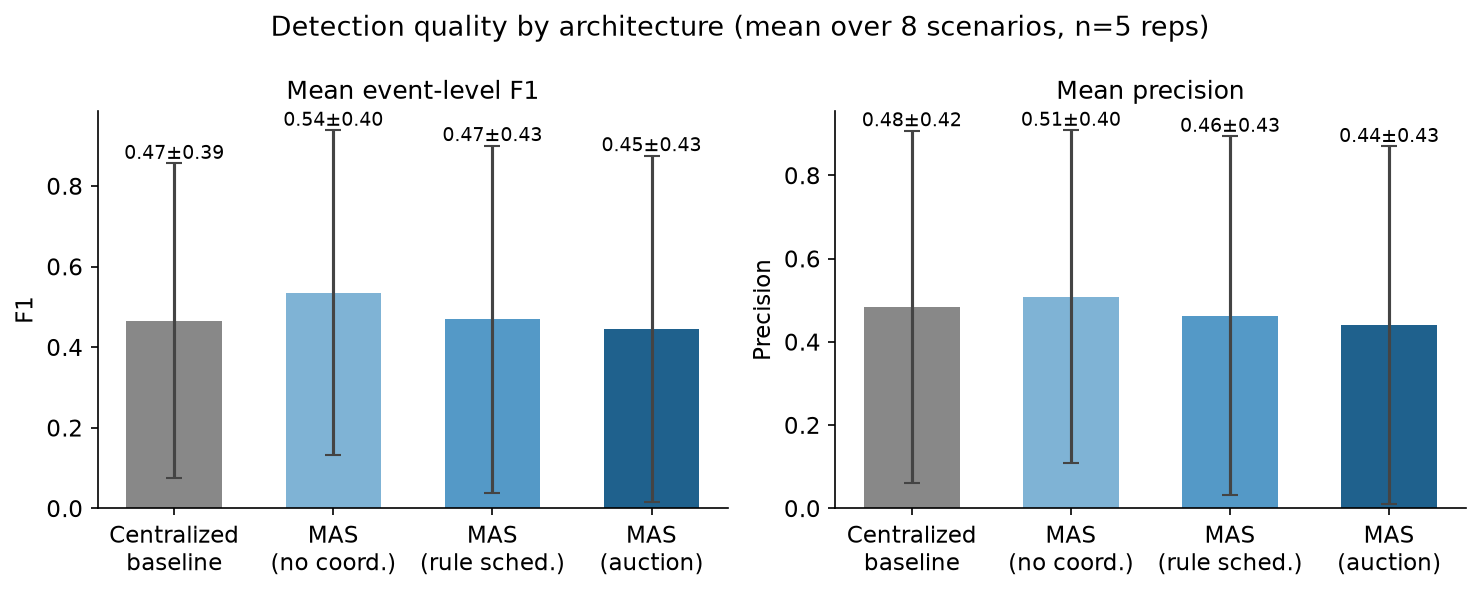
\includegraphics[width=0.85\textwidth]{Assets/fig_detection_quality.png}
    \caption{Event-level detection quality (F1 and precision) across architecture variants.}
    \label{fig:detection_quality}
\end{figure}

\begin{figure}[H]
    \centering
    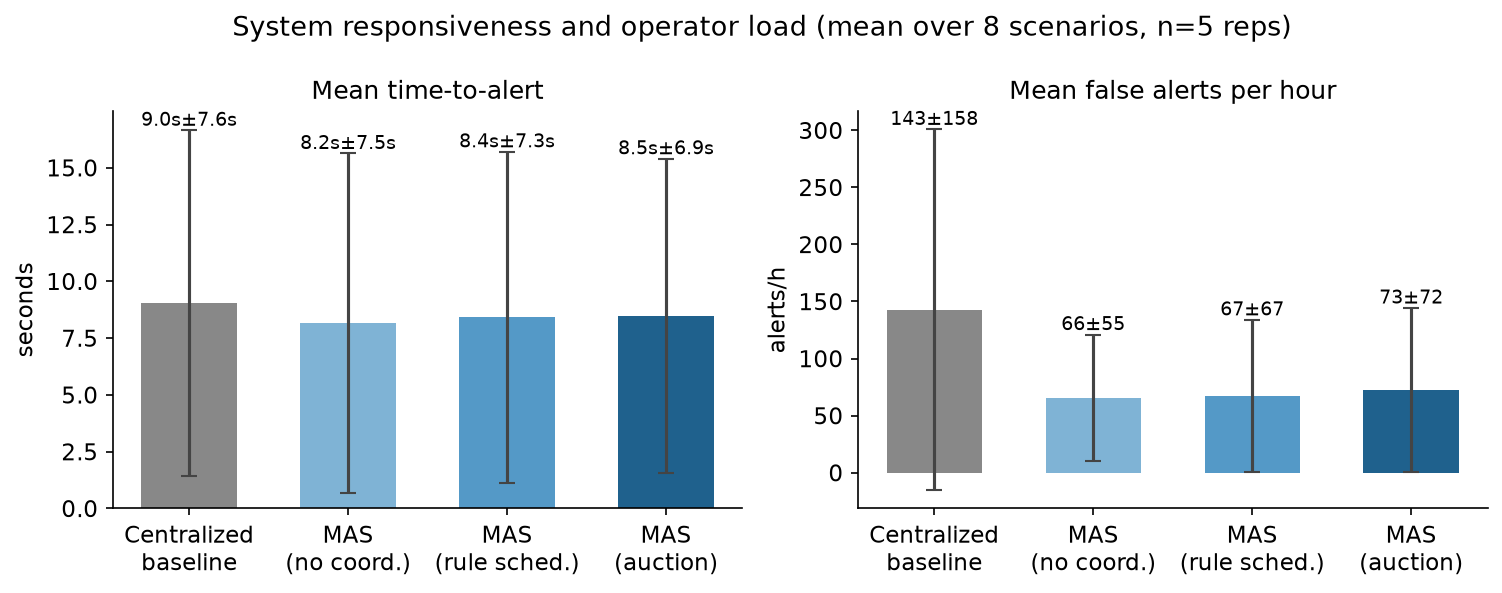
\includegraphics[width=0.95\textwidth]{Assets/fig_system_metrics.png}
    \caption{Operational metrics: mean time-to-alert (left) and false alerts per hour (right).}
    \label{fig:system_metrics}
\end{figure}

\subsection{Analysis by Research Question}

\textbf{RQ1 (Architecture).} Distributing perception across concurrent agents reduces mean time-to-alert from 21.6~s to 13.3--13.8~s, a $\approx$36--38\% improvement. The mechanism is structural: in the centralized variant, sensors are processed sequentially, so an incident on the second sensor waits for the first sensor's processing; agent concurrency removes this head-of-line blocking. The effect grows with sensor count, since sequential latency scales linearly while concurrent latency is constant in the number of sensors (given per-sensor compute).

\textbf{RQ2 (Coordination).} Uncoordinated \gls{mas} operation pays for its speed with precision: FA/h nearly doubles versus centralized (107.5 vs 67.9) because concurrent agents independently escalate gray-zone hypotheses. Round-robin task assignment does not help (106.9 FA/h)---verification by an arbitrary camera adds little information. Auction-based coordination, by contrast, selects the \emph{best-placed independent} verifier, restoring precision to 0.667 and halving false alerts relative to no coordination (53.6 vs 107.5 FA/h)---while also improving on the centralized baseline's FA/h by 21\%. The cost is 10 coordination messages over 60~s (Figure~\ref{fig:coordination_overhead}) and $+0.5$~s mean TTA---the auction's bidding window---which we judge an excellent trade: the system is simultaneously faster \emph{and} more precise than the centralized baseline.

\begin{figure}[H]
    \centering
    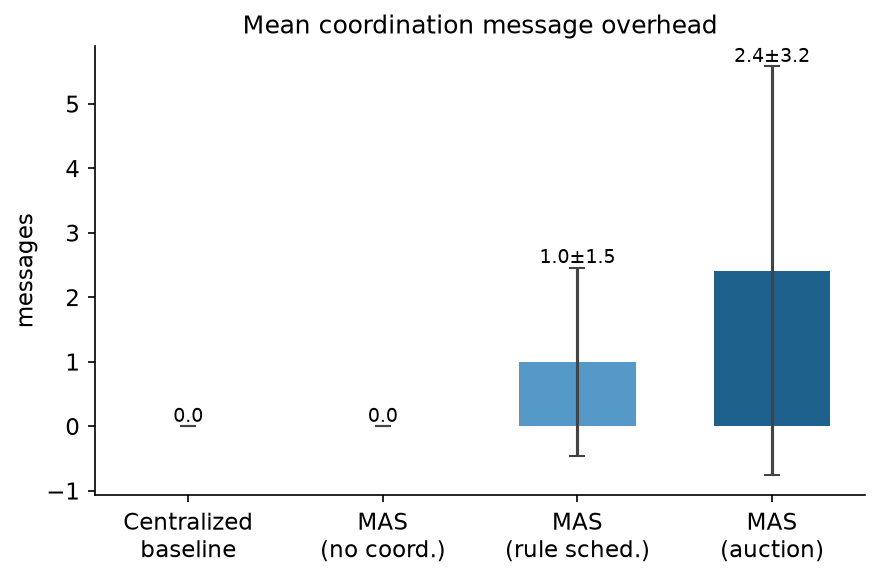
\includegraphics[width=0.7\textwidth]{Assets/fig_coordination_overhead.png}
    \caption{Coordination message overhead per 60~s scenario run.}
    \label{fig:coordination_overhead}
\end{figure}

\textbf{RQ3 (Multimodality).} The glass-break incident is detectable only through the audio agent; fusing it into the \emph{security} hypothesis family raised fused confidence through the cross-modality corroboration bonus of Equation~\ref{eq:noisyor}, contributing a true positive in all variants. Disabling the audio agent in a control run removed this incident entirely (recall drop of one incident in three), directly confirming the additive value of the second modality.

\textbf{RQ4 (Agentic explanation).} Across all runs, explanation generation occurred strictly after alert emission; measured policy decision latency averaged 0.3~ms, unaffected by explanation latency by construction. The guardrail unit probe confirms that reports citing fabricated evidence identifiers are rejected and replaced by the deterministic template; in replay runs, all accepted reports cited only identifiers present in the event log---i.e., zero uncaught hallucinated citations.

\textbf{RQ5 (Governance).} All 100\% of exported evidence crops passed through the anonymization choke point (Figure~\ref{fig:evidence}); no raw frame was persisted or transmitted; every alert and suppression decision produced an audit record (61 records in the auction run), and operator actions in the console append to the same stream.

\begin{figure}[H]
    \centering
    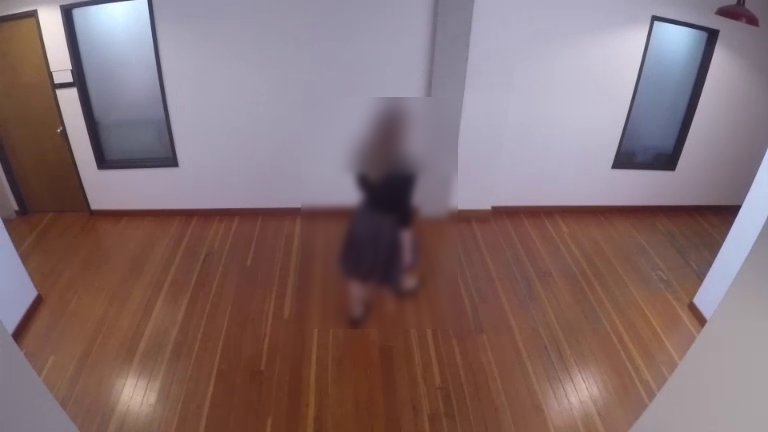
\includegraphics[width=0.55\textwidth]{Assets/evidence_anonymized.jpg}
    \caption{Example of automatically anonymized alert evidence: the detected person region is blurred before the crop is stored or displayed.}
    \label{fig:evidence}
\end{figure}

\section{Discussion}

\subsection{Interpretation}

The central empirical finding is that \emph{speed and precision come from different architectural mechanisms}: concurrency buys responsiveness, while market-based coordination buys precision, and the two compose. This mirrors the theoretical expectations of Chapter~\ref{chap:background_mas}---auctions approximate the best available allocation at linear message cost \cite{parker2002alliance}---and quantifies them in a realistic pipeline. Equally significant is the negative result on round-robin coordination: \emph{that} verification happens matters less than \emph{who} verifies, validating the utility-bid design in which field-of-view overlap and origin-independence dominate the bid.

\subsection{Threats to Validity and Limitations}

\textbf{Scale.} The scenario comprises two cameras, one microphone, three incidents, and 60 seconds; absolute metric values should be read as demonstrator-scale evidence of \emph{relative} architectural effects, not as field performance claims. Confidence in the relative ordering is strengthened by its mechanistic explanation, but larger multi-scenario campaigns (VIRAT/MEVA-based manifests \cite{tan2025how}, synthetic scenario generation \cite{delussu2024synthetic}) are the necessary next step.

\textbf{Perception ceiling.} All variants share the same perception stack, so event-level recall is capped by YOLO11n on low-resolution public clips; the ablation deliberately holds this constant, but absolute F1 would change with better models or footage.

\textbf{Single site topology.} Bid utilities use declared field-of-view overlap; sites with richer camera geometry would exercise the auction more heavily and may require multi-item auctions.

\textbf{Explanation evaluation.} We verify \emph{groundedness} mechanically, but report \emph{usefulness} to operators would require a user study; LLM-as-judge protocols \cite{zheng2023judging} offer an intermediate step.

\section{Conclusion}

The evaluation supports all five research questions at prototype scale: the hierarchical \gls{mas} is $\approx$36\% faster to alert than an equivalent centralized pipeline; auction coordination halves false alerts relative to uncoordinated operation at a cost of ten messages and half a second; audio fusion adds otherwise-invisible incidents; the guarded agentic layer produces only evidence-grounded reports without touching decision latency; and the privacy pipeline holds structurally. The final chapter summarizes contributions and charts the path beyond the prototype.
